\let\negmedspace\undefined
\let\negthickspace\undefined
\documentclass[journal]{IEEEtran}
\usepackage[a5paper, margin=10mm, onecolumn]{geometry}
%\usepackage{lmodern} % Ensure lmodern is loaded for pdflatex
\usepackage{tfrupee} % Include tfrupee package

\setlength{\headheight}{1cm} % Set the height of the header box
\setlength{\headsep}{0mm}     % Set the distance between the header box and the top of the text

\usepackage{gvv-book}
\usepackage{gvv}
\usepackage{cite}
\usepackage{amsmath,amssymb,amsfonts,amsthm}
\usepackage{algorithmic}
\usepackage{graphicx}
\usepackage{textcomp}
\usepackage{xcolor}
\usepackage{txfonts}
\usepackage{listings}
\usepackage{enumitem}
\usepackage{mathtools}
\usepackage{gensymb}
\usepackage{comment}
\usepackage[breaklinks=true]{hyperref}
\usepackage{tkz-euclide} 
\usepackage{listings}
% \usepackage{gvv}                                        
\def\inputGnumericTable{}                                 
\usepackage[latin1]{inputenc}                                
\usepackage{color}                                            
\usepackage{array}                                            
\usepackage{longtable}                                       
\usepackage{calc}                                             
\usepackage{multirow}                                         
\usepackage{hhline}                                           
\usepackage{ifthen}                                           
\usepackage{lscape}
\begin{document}

\bibliographystyle{IEEEtran}
\vspace{3cm}

\title{1.2.12}
\author{EE24BTECH11020 - Ellanti Rohith
}
% \maketitle
% \newpage
% \bigskip
{\let\newpage\relax\maketitle}

\renewcommand{\thefigure}{\theenumi}
\renewcommand{\thetable}{\theenumi}
\setlength{\intextsep}{10pt} % Space between text and floats


\numberwithin{equation}{enumi}
\numberwithin{figure}{enumi}
\renewcommand{\thetable}{\theenumi}


\textbf{Question}:\vspace{.5em} \\ If \myvec{1 \\ 2}, \myvec {4 \\ y}, \myvec{x \\ 6} and \myvec{3 \\ 5} are the vertices of parallelogram taken in order, find $x$ and $y$.\vspace{.5em} \\  \textbf{Solution:} \\ \hspace {0.5em} Let ABCD be the given Parallelogram, \\ 
\begin{table}[h!]
\centering
    \caption{Coordinates of the vertices of parallelogram ABCD}
\begin{tabular}[12pt]{ |c| c|}
    \hline
    \textbf{Variable} & \textbf{Description}\\ 
    \hline
	$\vec{e}$ & Eccentricity of conic\\
	\hline
	$\vec{F}$ & Focus of conic\\
	\hline
	$\vec{I}$ & Identity matrix\\
	\hline
	$\vec{n}^{\top}\vec{x}=c$ & Equation of directrix\\
	\hline
	$\vec{n}$ & Slope of normal to directrix\\
	\hline
	$f$ & $\norm{\vec{n}}^2\norm{\vec{F}}^2-c^2e^2$\\
	\hline
	$\vec{V}$ & A symmetric matrix given by eigenvalue decomposition\\
	\hline
	$\vec{u}$ & Vertex of conic with same directrix\\
	\hline
\end{tabular}

\end{table}
 \\ we know that $\vec{AB}$ is parallel to $\vec{DC}$ and  $\abs{\abs{AB}}$ $=$ $\abs{\abs{DC}}$ \\ Then,
\begin{align}
	\vec{B}-\vec{A}&=\vec{C}-\vec{D}\\[.5em]
\myvec{4 \\ y}-\myvec{1 \\ 2}&=\myvec{x \\ 6}-\myvec{3 \\ 5}\\[0.5em] 
\myvec{3 \\ y-2}&=\myvec{x-3 \\ 1}\label{eq1.2.12.1} \end{align}
\hspace{8em} From equation\hspace{0.5em} \eqref{eq1.2.12.1}, \begin{align} &3=x-3	\Rightarrow x=6  \end{align} \begin{align} &y-2=1 \Rightarrow y=3\end{align}
\begin{figure}[h!]
   \centering 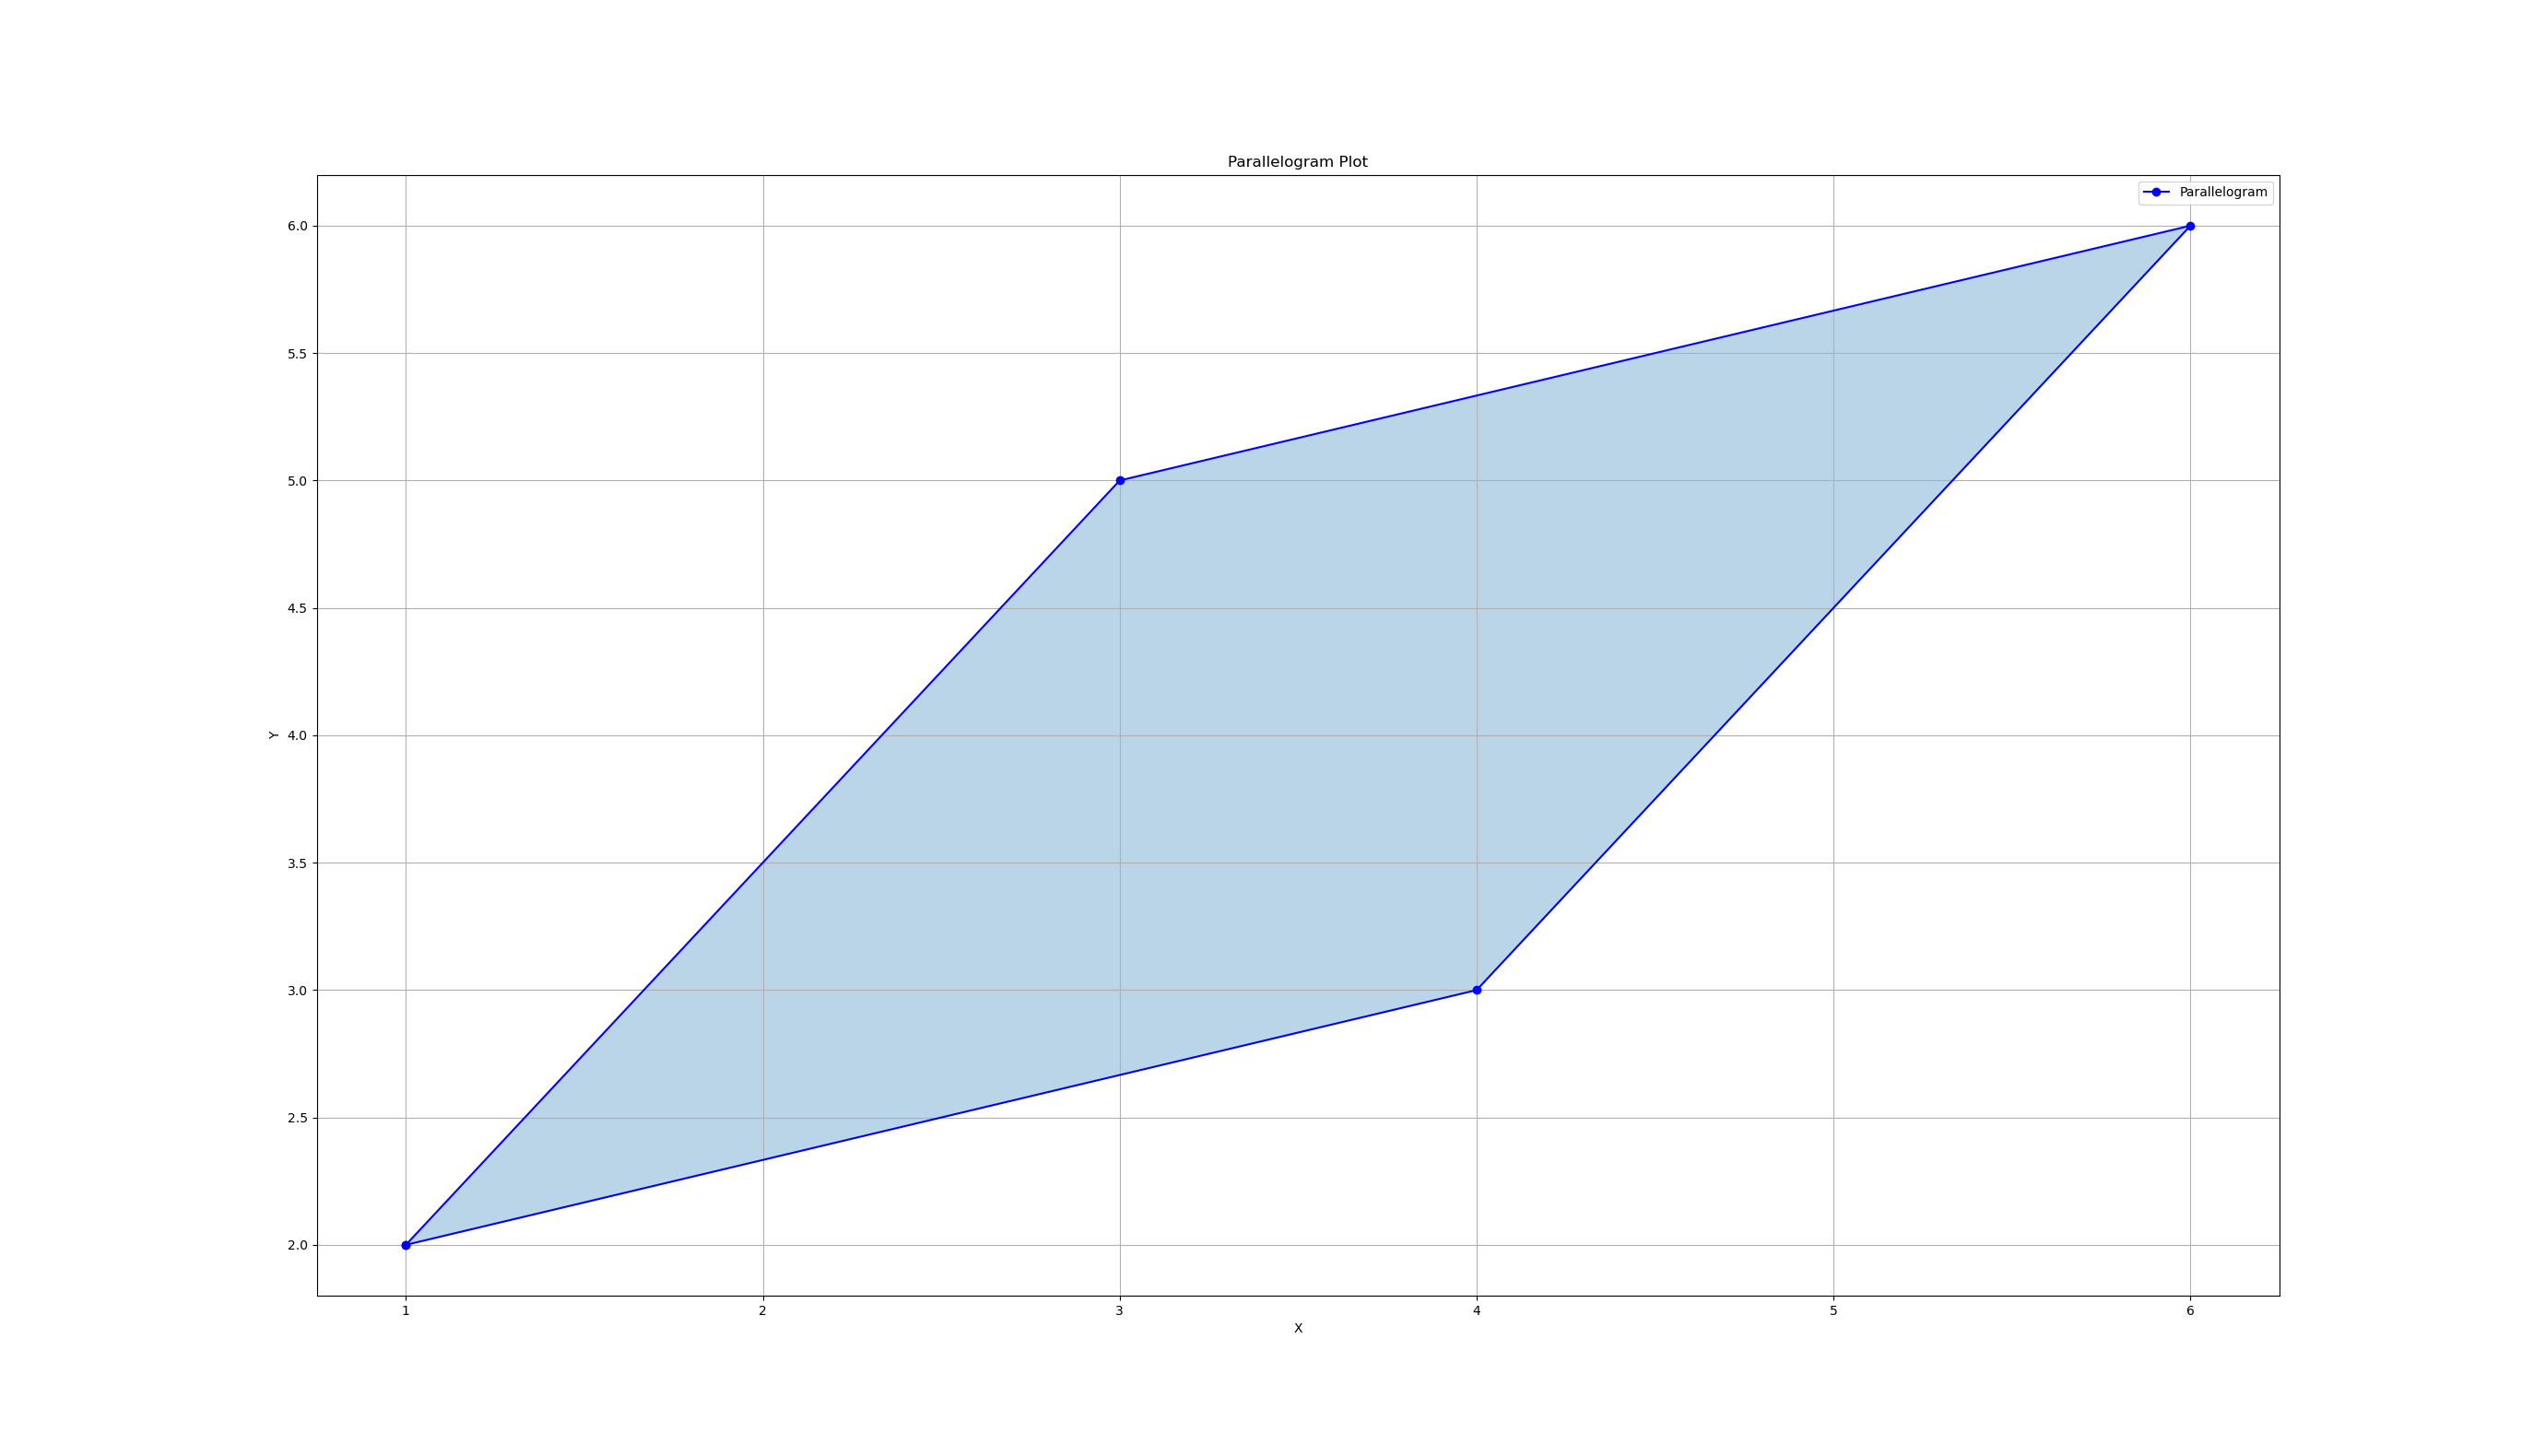
\includegraphics[width=0.7\linewidth]{figs/Figure_1.png}
   \caption{Plot of parallelogram ABCD}
   \label{Parallelogram}
\end{figure}
\end{document}

